%\documentclass[onecolumn]{IEEEtranTIE}
\documentclass[journal]{IEEEtranTIE}
\usepackage{graphicx}
\usepackage{cite}
\usepackage{picinpar}
\usepackage{amsmath}
\usepackage{url}
\usepackage{flushend}
\usepackage[latin1]{inputenc}
\usepackage{colortbl}
\usepackage{soul}
\usepackage{multirow}
\usepackage{pifont}
\usepackage{color}
\usepackage{alltt}
\usepackage[hidelinks]{hyperref}
\usepackage{enumerate}
\usepackage{siunitx}
\usepackage{breakurl}
\usepackage{epstopdf}
\usepackage{pbox}

\begin{document}
\title{	ConAuth - context for authentication \\ (Dec. 2017)}

\author{
	\vskip 1em
	{
	Saurabh Sharma, \emph{saurabh.sharma@sv.cmu.edu}\\
	Omar Serrano, \emph{omar.serrano@sv.cmu.edu}
	}
}

\maketitle

\begin{abstract}
With the growing number of wireless devices, we need efficient mechanisms to let
the wireless devices communicate securely. The wireless devices sometimes share
common sensors that can be leveraged to perform additional authentication
procedures on a set of localized wireless devices. The problem which prevents
such a judicious use of sensors is the orientation of wireless devices. Sensors
such as gyroscope and accelerometer are commonly found in wireless devices, but
their readings make no sense until their orientations are the same. We plan to
conduct controlled experiments to investigate how different environmental factors
impact the accelerometer performance and how the best accuracy can be achieved
in an appropriate condition range. We also characterize the nature of an
accelerometer to understand its performance in different conditions. Based on
such comprehensive understanding, we propose to estimate the phone attitude and
provide for opportunistic calibration of the accelerometer
\end{abstract}

\begin{IEEEkeywords}
Contextual security, sensor funsion, Madgwick, device orientation.
\end{IEEEkeywords}

\definecolor{limegreen}{rgb}{0.2, 0.8, 0.2}
\definecolor{forestgreen}{rgb}{0.13, 0.55, 0.13}
\definecolor{greenhtml}{rgb}{0.0, 0.5, 0.0}

\section{Introduction}

\IEEEPARstart{W}{ith}
the growing number of IoT devices, securely pairing a new device into an
existing set of devices is an extremely important yet burdensome task.
Traditionally, these devices are paired manually, where an operator sets up an
authentication with the existing network of devices. Specifically, we address
the problem of a platoon ghost attack wherein an attacker device spoofs presence
within a platoon to gain admission and subsequently execute malicious attacks
\cite{Han}. To address such concerns, we explore the notion of fingerprinting
device sensor readings for a device's context.

Devices that share context are expected to experience similar events. For
example, two magnetometers in proximity are likely to processes similar events
if a magnetic strip is drawn close to them. Even if the readings are not exactly
the same, the devices are likely to exhibit similar patterns as a result of the
magnetic disturbance caused by the magnetic strip. Two video cameras, despite
having different points of view, might be able to determine that they share
context on the basis that both of them detect an object with similar shape and
color; for example, if one of the video cameras records an invidual with a blue
shirt walking toward it, and the other camera records an invidual with a blue
shirt walking away from it.

There is a wide range of possibilities in how devices and sensors are used to
determine context from a wide variety of physical stimuli, or how the scale of
context is defined (e.g., school building vs a single room); however, we limit
our research to the small context of a car, and to 3-dimensional orientation,
acceleration, and magnetic sensor readings.

\section{Problem Statement}

With near-ubiquitous availability of wireless devices equipped with a wide
variety of sensors, research in building context aware services has been
growing. However, despite a large number of services proposed and developed as
research prototypes, the number of truly context-aware applications available in
wireless devices is quite limited. A major barrier for the large-scale
proliferation of context aware applications is poor accuracy \cite{Alanezi}.
We address one of the key reasons for this poor accuracy, which is the impact of
sensor orientation.

Devices have their sensors oriented in different positions. We first show that
smartphone positions significantly affect the values of the
sensor data being collected by a context aware application, and this in turn
has a significant impact on the accuracy of the application \cite{Alanezi}.
Next, it describes the design and prototype development of a orientation
discovery service that accurately detects a sensor orientation. This service is
based on the sensor data collected from carefully chosen sensors. Finally, the
paper demonstrates that the accuracy of an existing context aware service or
application is significantly enhanced when run in conjunction with the proposed
orienttion discovery service.


\begin{figure}[!t]\centering
	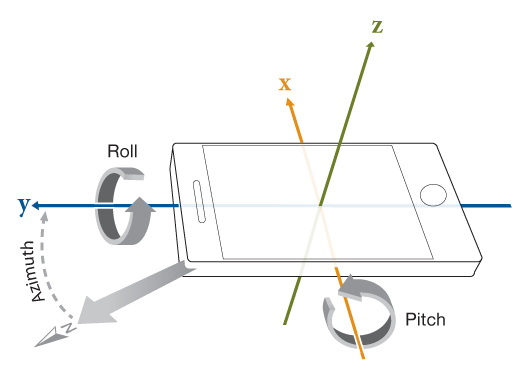
\includegraphics[width=8.5cm]{phoneOrientation}
	\caption{A device's body orientation.}\label{fig:fig1}
\end{figure}


\section{Technical Approach}

The process to determine whether two devices share the same context consists of
the following steps:

\begin{enumerate}
\item Determining the orientation of the devices in question.
\begin{enumerate}
\item Obtain sensor data from PowerDue with a sensor that contains a gyroscope,
      and possibly an accelerometer.
\item Obtain sensor data from a mobile phone using iOS app PowerSense. See
      Figure~\ref{fig:fig2} and Figure~\ref{fig:fig3} for an example of the type
      of data that may be collected with PowerSense.
\item Compute orientation difference using Madgwick algorithm.
\end{enumerate}
\item Correlating the sensor data to determine whether sensors share context.
\end{enumerate}

2 depends on 1, because knowing the orientation, or attitude, of two devices
allows us take the difference between a devices body-orientation, as depicted in
Figure~\ref{fig:fig1}, with respect to the geoframe, the earth's orientation. Existing
algorithms, as described in the next two subsections, can determine the
orientation, but we've chosen to use Madgwick because it is open source and well
suited for small embedded devices \cite{Madgwick}. The purpose of our remaining
work is to determine 2, a technique for correlating data between two or more
devices to allow us to determine shared context.

\subsection{Computing the attitude of a device}

The phone attitude is obtained by doing continuos integration on the angular
velocity, and by taking the difference between the geoframe, the earth
coordinate sytem, and the body-frame, the coordinate system of the device's
body. Per \cite{PhoneAttitude}, the best approach for calculating the difference
between both coordinate systems is the Euler Axis/Angle method, which solves the
problem from the geoframe's perspective. To compute the integration, the total
device motion is split into multiple time windows, and the rotation of the
device is the accumulated rotation of all the time windows.

\begin{figure}[!t]\centering
	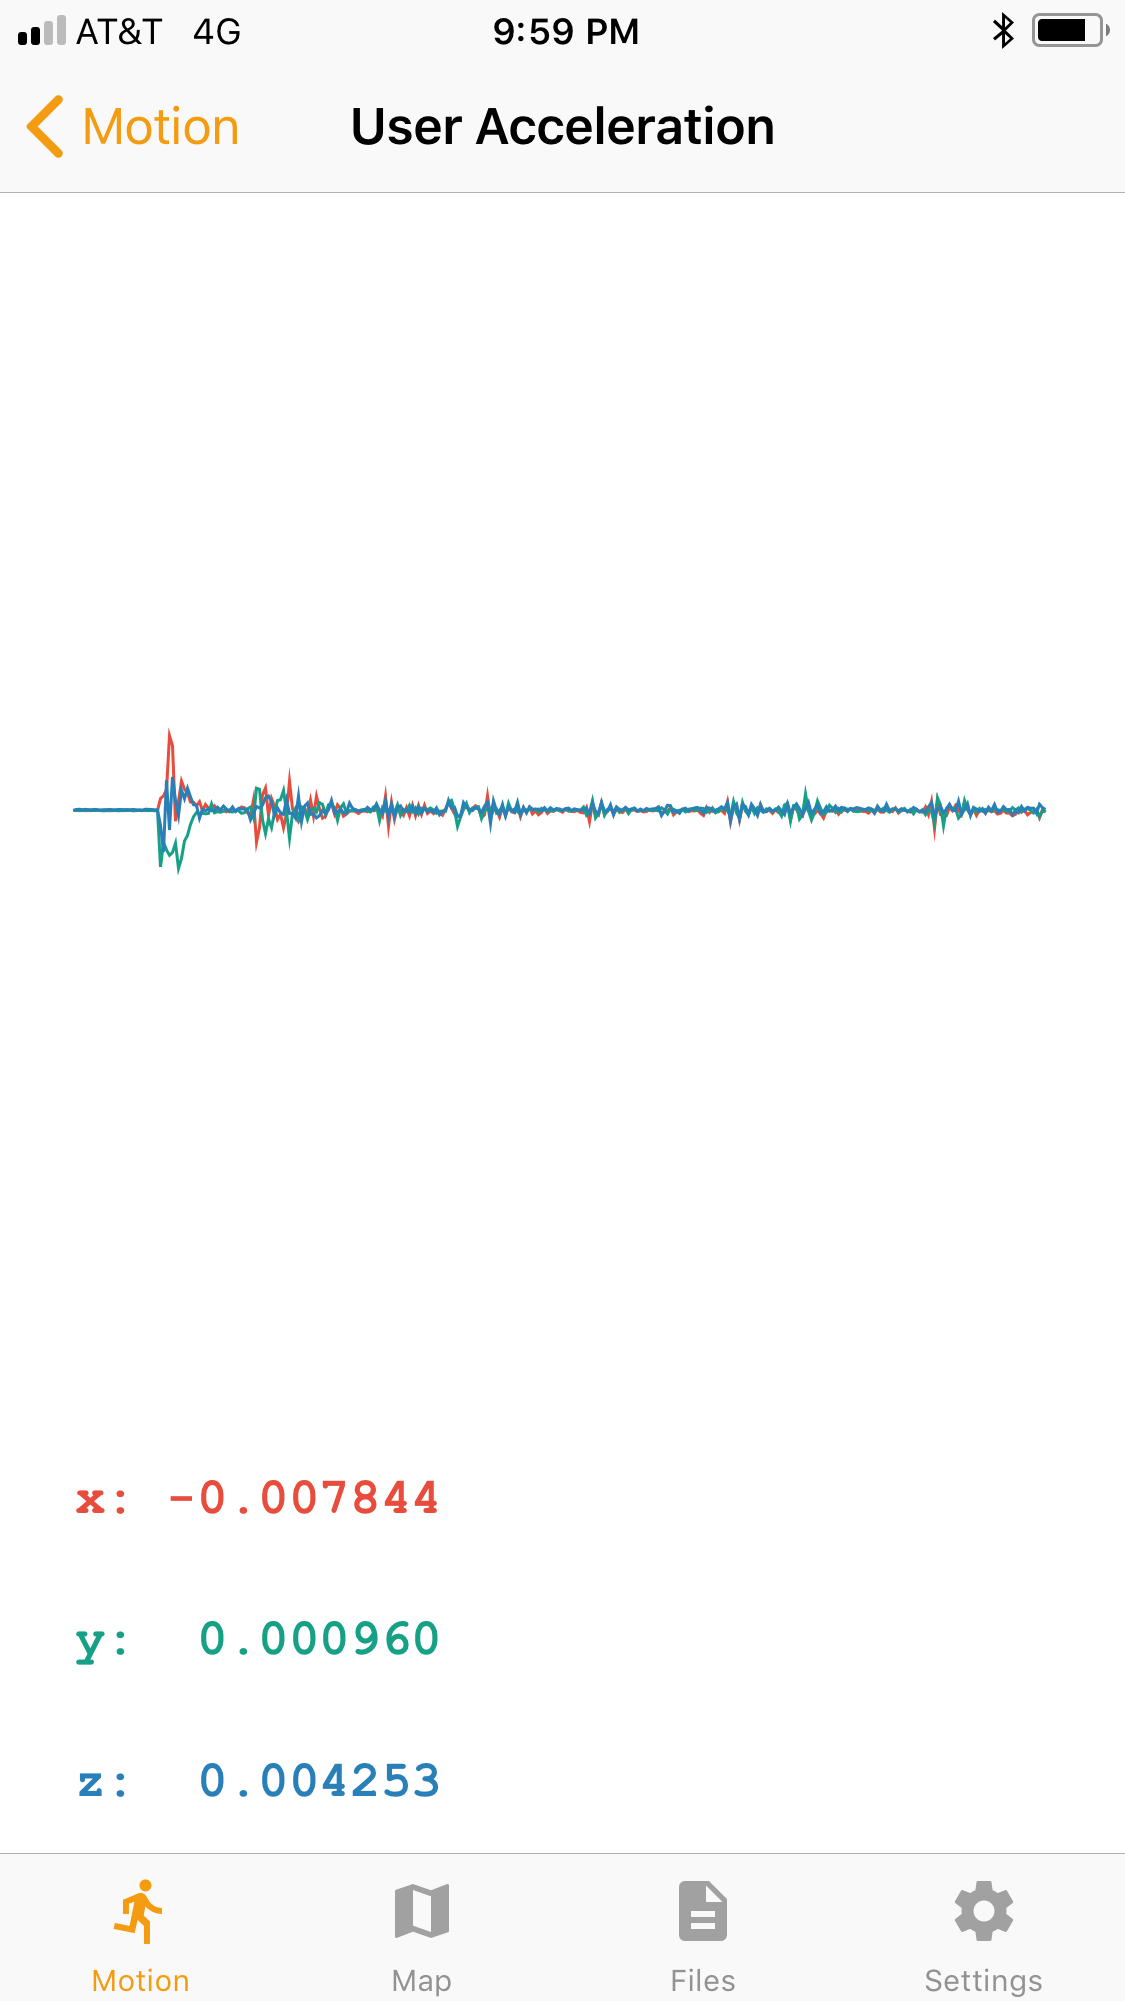
\includegraphics[width=5.5cm]{acceleration}
	\caption{User acceleration with iOS app PowerSense.}\label{fig:fig2}
\end{figure}

\subsection{Madgwick algorithm}

Historically, the Kalman filter, and other techniques, including fuzzy
processing and frequency domain filters, have been used as the basis for
orientation algorithms; however, these techniques have several disadvantages
\cite{Madgwick}. For example, the Kalma filter is computationally expensive,
and some of the other techniques are only effective under limited conditions
\cite{Madgwick}. Therefore, we plan to use Madgwick, an algorithm that employs a
quaternion representation of orientation, which has had positive results despite
the fact that it does not require the heavy computational load, or high
frequency sampling of a Kalman-filter based algorithm \cite{Madgwick}.

\section{Pending work}

Up until this point, our work has consisted of research, and more of it
remains to be done; however, there are key steps that we need to follow through
with in order to deliver results on the research:

\begin{enumerate}
\item Obtain a sensor with a gyroscope and accelerometer. None of the sensor at
      our disposal contain a gyroscope, which is the center piece of
      orientation-sensing algorithms. Therefore, it is imperative that we obtain
      one soon, because using a new sensor might entail having to modify or
      create drivers for the PowerDue.
\item Compute the attitude of the PowerDue.
\item Compute the attidue of a mobile phone.
\item Correlate the readings from the PowerDue and mobile phone.
\end{enumerate}

Our plan is to run experiments in which we repeat steps 2 - 4 under different
conditions, but in all the PowerDue and the mobile phone are stationary when the
sensor data is collected:

\begin{itemize}
\item Both devices have the same orientation and are in the same context.
\item Both devices are in the same context, but their orientations differ.
\item Devices are not in the same context, but have the same orientation.
\item Devices are not in the same context, and have different orientations.
\end{itemize}

To deliver useful results, we have to correlate the data between different
devices, and define what it means for two devices to share context. Also note
that we plan to correlate the data between the devices by doing the
analysis on our PCs, but ideally it would be more useful to deploy the model
on the PowerDue, perhaps a task for future work.

\begin{figure}[!t]\centering
	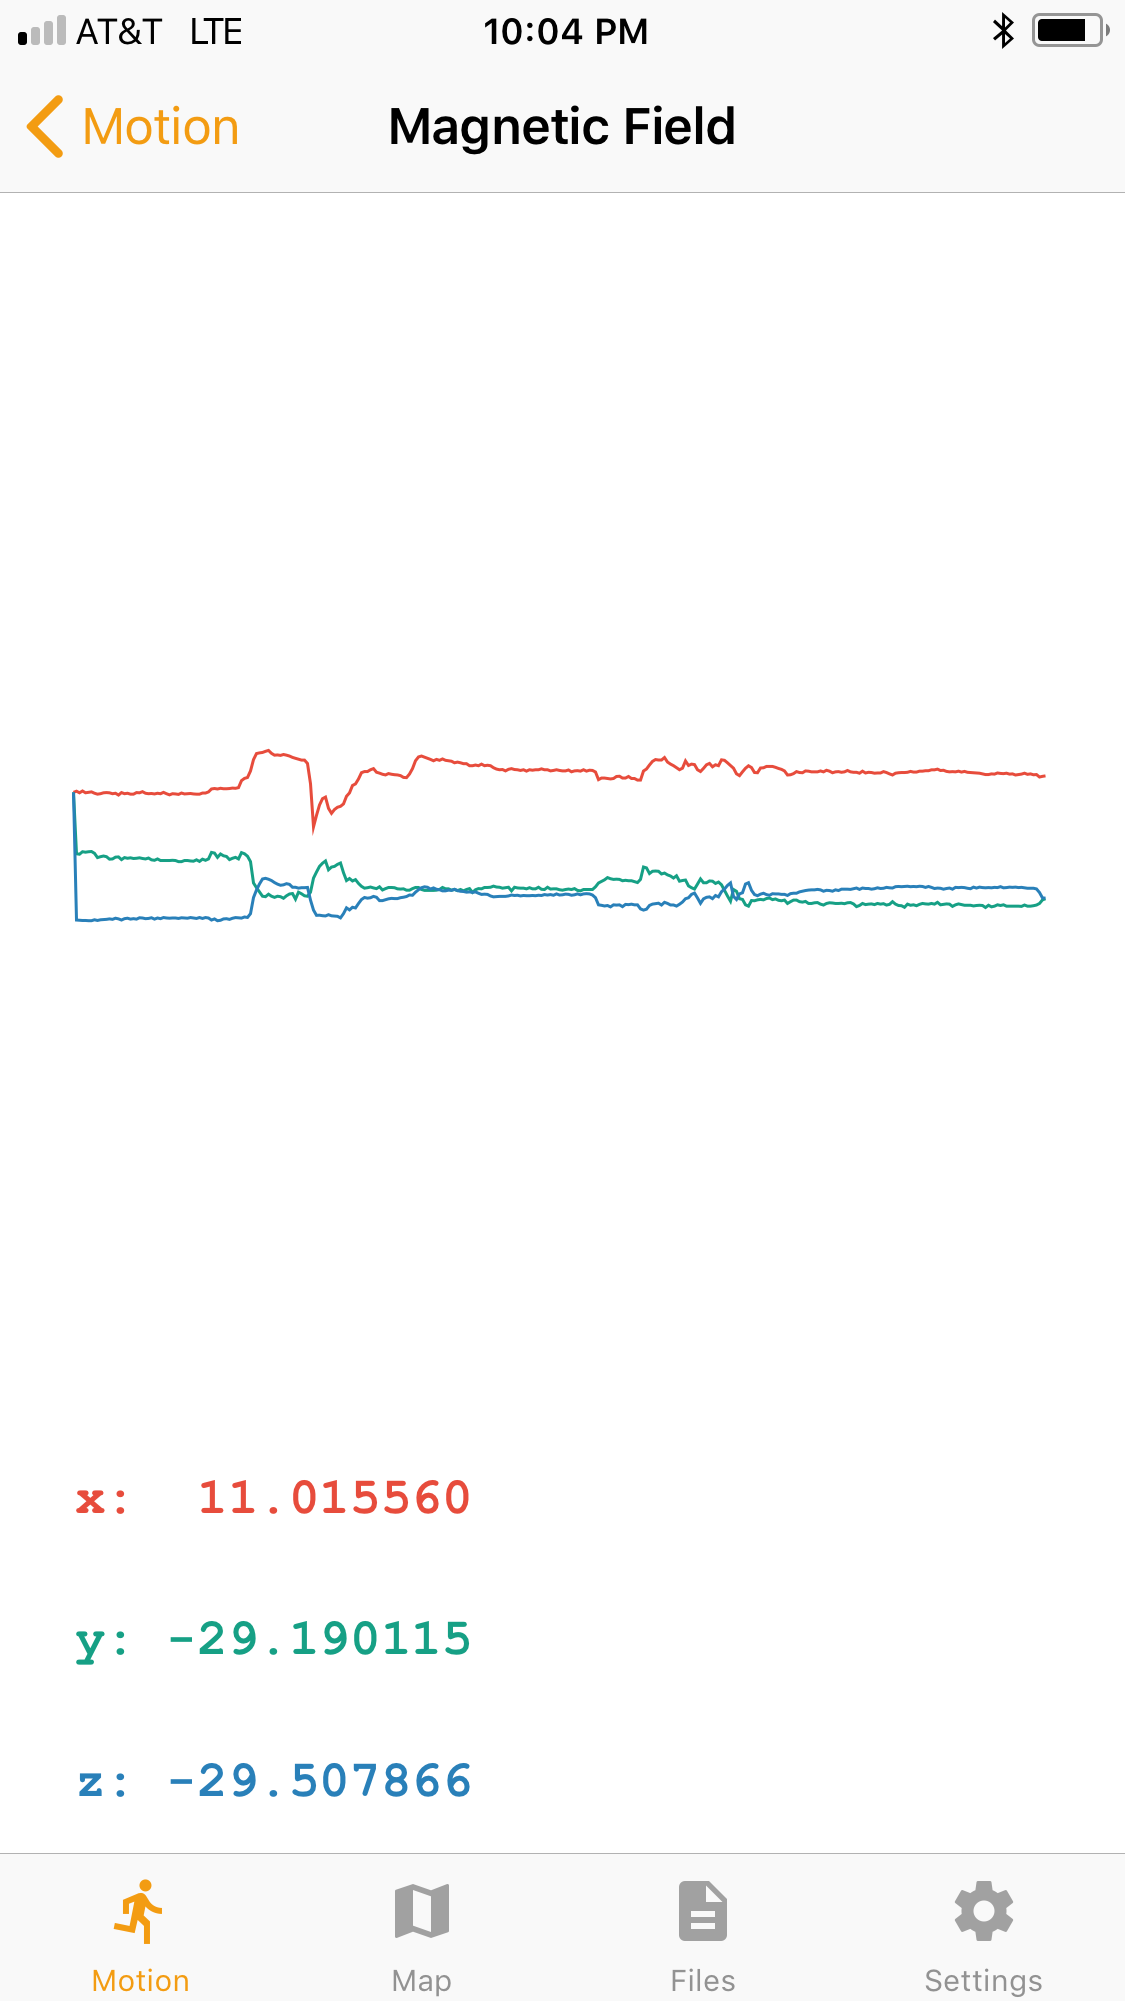
\includegraphics[width=5.5cm]{magnetic_field}
	\caption{Magnetic field with iOS app PowerSense.}\label{fig:fig3}
\end{figure}

% References

\bibliographystyle{Bibliography/IEEEtranTIE}
\bibliography{Bibliography/IEEEabrv,Bibliography/BIB_1x-TIE-2xxx}\ %IEEEabrv instead of IEEEfull

\end{document}
